\chapter{Methodology}
\label{ch:method}

This chapter describes the methodology used to develop the UnFake fake news detection system. It covers the datasets used for training, the machine learning models developed, the system architecture, and the implementation details.

\section{System Overview}
\label{sec:system_overview}

The UnFake system uses a dual-model approach to classify news content as real or fake. Two separate models are used to handle different types of content:

\begin{enumerate}
    \item \textbf{Headline Model:} A fine-tuned RoBERTa transformer for classifying short statements and headlines (up to 256 tokens).
    
    \item \textbf{Article Model:} A Gradient Boosting Classifier with TF-IDF vectorization for classifying full-length news articles.
\end{enumerate}

This approach allows the system to optimize performance for each content type. Short statements require a model that can understand context from limited text, while longer articles provide more features for traditional machine learning approaches.

Figure~\ref{fig:system_architecture} shows the overall system architecture.

\begin{figure}[!ht]
    \centering
    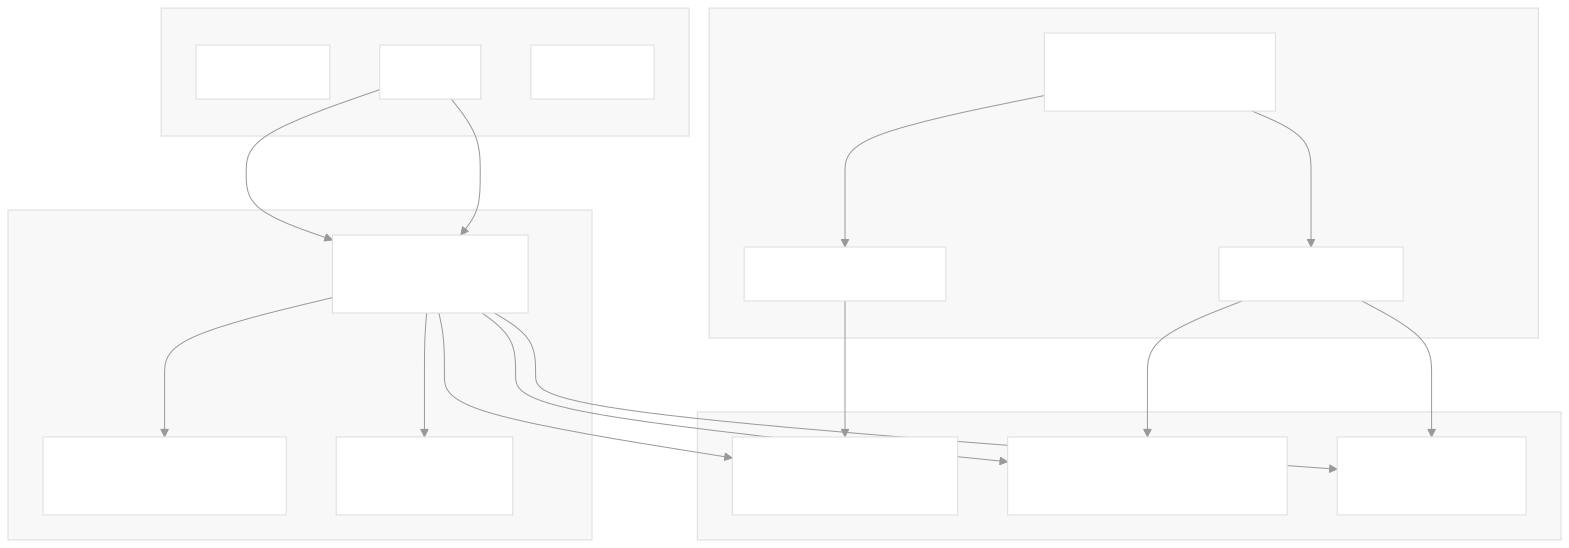
\includegraphics[width=0.9\textwidth]{figures/System Component Architecture.svg}
    \caption{System Component Architecture showing the three-tier structure of the UnFake system.}
    \label{fig:system_architecture}
\end{figure}

\section{Datasets}
\label{sec:datasets}

Multiple datasets were used to train the models in this project.

\subsection{Headline Model Dataset}
\label{subsec:headline_dataset}

The headline model was trained on fact-checked statements from PolitiFact, a Pulitzer Prize-winning fact-checking organization. A web scraper was developed to collect statements and their verdicts from the PolitiFact website.

The dataset contains statements with the following verdicts:
\begin{itemize}
    \item True
    \item Mostly True
    \item Half True
    \item Mostly False
    \item False
    \item Pants on Fire
\end{itemize}

For binary classification, these verdicts were mapped to two classes as shown in Figure~\ref{fig:label_mapping}:
\begin{itemize}
    \item \textbf{Real (1):} True, Mostly True, Half True
    \item \textbf{Fake (0):} Mostly False, False, Pants on Fire
\end{itemize}

\begin{figure}[!ht]
    \centering
    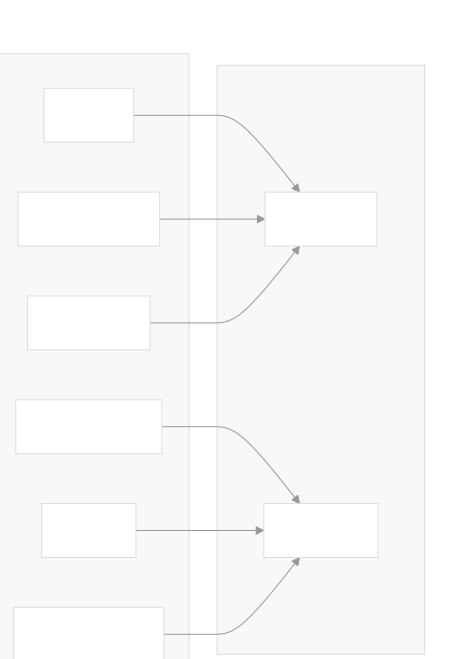
\includegraphics[width=0.7\textwidth]{figures/Headline Model Dataset Label Mapping.svg}
    \caption{Label mapping for the headline model dataset.}
    \label{fig:label_mapping}
\end{figure}

After preprocessing, the dataset contained \textbf{25,999 statements}. The class distribution was imbalanced, with more fake statements than real ones. Class weights were computed to handle this imbalance during training.

\subsection{Article Model Dataset}
\label{subsec:article_dataset}

The article model was trained on a dataset of news articles containing:
\begin{itemize}
    \item \textbf{True.csv:} Collection of real news articles
    \item \textbf{Fake.csv:} Collection of fake news articles
\end{itemize}

The combined dataset contains \textbf{44,898 articles}, split into training (75\%) and testing (25\%) sets.

\section{Data Preprocessing}
\label{sec:preprocessing}

Text preprocessing is an important step that prepares the raw text data for the machine learning models.

\subsection{Headline Model Preprocessing}
\label{subsec:headline_preprocessing}

For the headline model, the following preprocessing steps are applied:

\begin{lstlisting}[language=Python, caption={Text preprocessing function for headlines}, label=list:clean_text]
def clean_text(text: str) -> str:
    text = text.lower()
    text = re.sub(r"[^a-z0-9\s,.!?]", " ", text)
    text = re.sub(r"\s+", " ", text)
    text = text.strip()
    return text
\end{lstlisting}

The preprocessing steps include:
\begin{enumerate}
    \item Converting text to lowercase
    \item Removing special characters except basic punctuation
    \item Normalizing whitespace
    \item Stripping leading and trailing whitespace
\end{enumerate}

Additionally, Spanish language statements were removed from the dataset to focus on English content.

\subsection{Article Model Preprocessing}
\label{subsec:article_preprocessing}

For the article model, more aggressive preprocessing is applied:

\begin{lstlisting}[language=Python, caption={Text preprocessing function for articles}, label=list:clean_article]
def clean_article(text: str) -> str:
    text = text.lower().strip()
    text = re.sub(r"https?://\S+|www\.\S+", "", text)
    text = re.sub(r"\[.*?\]", "", text)
    text = re.sub(r"\w*\d\w*", "", text)
    text = re.sub(r"<.*?>+", "", text)
    text = re.sub(r"\n", " ", text)
    text = re.sub(r"\s+", " ", text)
    text = re.sub(r"\W", " ", text)
    return text
\end{lstlisting}

The preprocessing steps include:
\begin{enumerate}
    \item Converting to lowercase
    \item Removing URLs
    \item Removing text in square brackets
    \item Removing words containing numbers
    \item Removing HTML tags
    \item Normalizing newlines and whitespace
    \item Removing non-word characters
\end{enumerate}

\section{Headline Model: RoBERTa}
\label{sec:headline_model}

The headline model uses a fine-tuned RoBERTa transformer for sequence classification.

\subsection{Model Architecture}
\label{subsec:headline_architecture}

RoBERTa (Robustly Optimized BERT Pretraining Approach) is a transformer-based language model. The architecture consists of:

\begin{itemize}
    \item \textbf{Embedding layer:} Converts tokens to dense vectors
    \item \textbf{Transformer encoder layers:} 12 layers with self-attention and feed-forward networks
    \item \textbf{Classification head:} Linear layer for binary classification
\end{itemize}

The model uses the \texttt{roberta-base} checkpoint from Hugging Face as the starting point, which is then fine-tuned on the PolitiFact dataset.

\subsection{Training Process}
\label{subsec:headline_training}

The training process involves:

\begin{enumerate}
    \item \textbf{Tokenization:} Text is tokenized using the RoBERTa tokenizer with a maximum length of 256 tokens. Shorter sequences are padded, and longer sequences are truncated.
    
    \item \textbf{Dataset split:} The data is split into 80\% training and 20\% test sets with stratification to maintain class balance.
    
    \item \textbf{Class weighting:} Computed class weights are used to handle the imbalanced dataset.
    
    \item \textbf{Optimization:} AdamW optimizer with learning rate scheduling (linear warmup followed by decay).
    
    \item \textbf{Training loop:} The model is trained for multiple epochs, with validation after each epoch.
\end{enumerate}

Figure~\ref{fig:headline_training} shows the training history including loss, accuracy, and F1 score over epochs.

\begin{figure}[!ht]
    \centering
    \includegraphics[width=\textwidth]{figures/Headline Model Training History (Loss, Accuracy, F1 Score).png}
    \caption{Headline model training history showing loss, accuracy, and F1 score over epochs.}
    \label{fig:headline_training}
\end{figure}

\subsection{Device Selection}
\label{subsec:device_selection}

The model automatically selects the best available device for inference:

\begin{lstlisting}[language=Python, caption={Device selection for model inference}, label=list:device]
DEVICE = torch.device("cuda" if torch.cuda.is_available() else "cpu")
\end{lstlisting}

When a GPU is available, it is used for faster inference. Otherwise, the model runs on CPU.

\section{Article Model: Gradient Boosting}
\label{sec:article_model}

The article model uses a Gradient Boosting Classifier combined with TF-IDF vectorization.

\subsection{TF-IDF Vectorization}
\label{subsec:tfidf}

TF-IDF (Term Frequency-Inverse Document Frequency) converts text documents into numerical feature vectors. For each word in a document:

\begin{equation}
\text{TF-IDF}(t, d) = \text{TF}(t, d) \times \text{IDF}(t)
\label{eq:tfidf}
\end{equation}

Where:
\begin{itemize}
    \item $\text{TF}(t, d)$ is the frequency of term $t$ in document $d$
    \item $\text{IDF}(t) = \log\frac{N}{n_t}$ where $N$ is the total number of documents and $n_t$ is the number of documents containing term $t$
\end{itemize}

The TF-IDF vectorizer learns the vocabulary from the training data and transforms both training and test data into the same feature space.

\subsection{Gradient Boosting Classifier}
\label{subsec:gradient_boosting}

The Gradient Boosting Classifier builds an ensemble of decision trees sequentially, with each tree correcting the errors of previous trees. Key parameters include:

\begin{itemize}
    \item Number of estimators (trees)
    \item Learning rate (shrinkage)
    \item Maximum tree depth
    \item Minimum samples per leaf
\end{itemize}

The model is trained on the TF-IDF transformed training data and achieves excellent performance on the test set.

\subsection{Model Comparison}
\label{subsec:model_comparison}

During development, several classification algorithms were evaluated:

\begin{figure}[!ht]
    \centering
    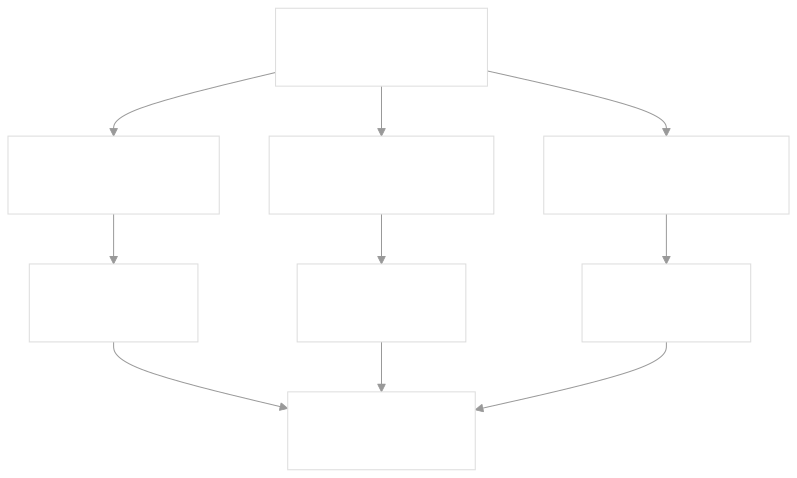
\includegraphics[width=0.8\textwidth]{figures/Article Model Multi-Model Evaluation.svg}
    \caption{Comparison of different classification algorithms for the article model.}
    \label{fig:model_comparison}
\end{figure}

The Gradient Boosting Classifier was selected as it provided the best balance of accuracy and performance.

\section{Backend API}
\label{sec:backend_api}

The backend API is built using FastAPI, a modern Python web framework for building APIs.

\subsection{API Structure}
\label{subsec:api_structure}

The API provides the following endpoints:

\begin{table}[!ht]
    \centering
    \caption{API Endpoints}
    \label{tab:api_endpoints}
    \begin{tabular}{llp{6cm}}
        \toprule
        Endpoint & Method & Description \\
        \midrule
        \texttt{/} & GET & Health check and model status \\
        \texttt{/predict} & POST & Single statement classification \\
        \texttt{/predict/batch} & POST & Batch statement classification (up to 100) \\
        \texttt{/predict/article} & POST & Single article classification \\
        \texttt{/predict/article/batch} & POST & Batch article classification (up to 50) \\
        \bottomrule
    \end{tabular}
\end{table}

\subsection{Request/Response Flow}
\label{subsec:request_flow}

Figure~\ref{fig:request_flow} shows the request/response flow through the API.

\begin{figure}[!ht]
    \centering
    \includegraphics[width=0.9\textwidth]{figures/RequestResponse Flow.svg}
    \caption{Request and response flow through the API.}
    \label{fig:request_flow}
\end{figure}

\subsection{Model Loading}
\label{subsec:model_loading}

Models are loaded at application startup using FastAPI's lifespan management:

\begin{lstlisting}[language=Python, caption={Model loading at startup}, label=list:lifespan]
@asynccontextmanager
async def lifespan(app: FastAPI):
    load_headline_model()
    load_article_model()
    yield
\end{lstlisting}

This ensures models are ready when the API starts receiving requests.

\section{Frontend Application}
\label{sec:frontend}

The frontend is a single-page web application built with HTML, CSS, and vanilla JavaScript.

\subsection{User Interface}
\label{subsec:user_interface}

The interface allows users to:
\begin{enumerate}
    \item Switch between statement and article analysis modes
    \item Enter text content for analysis
    \item View prediction results with confidence scores
    \item See probability breakdown for fake vs. real classification
\end{enumerate}

Figure~\ref{fig:frontend_input} shows the input interface, and Figure~\ref{fig:frontend_result} shows the results display.

\begin{figure}[!ht]
    \centering
    \includegraphics[width=0.8\textwidth]{figures/Frontend Screenshot Input Statement.png}
    \caption{Frontend interface for inputting statements.}
    \label{fig:frontend_input}
\end{figure}

\begin{figure}[!ht]
    \centering
    \includegraphics[width=0.8\textwidth]{figures/Frontend Screenshot Statement Result.png}
    \caption{Frontend display of classification results.}
    \label{fig:frontend_result}
\end{figure}

\subsection{API Communication}
\label{subsec:api_communication}

The frontend communicates with the backend API using fetch requests:

\begin{lstlisting}[language=JavaScript, caption={API communication in the frontend}, label=list:frontend_api]
const endpoint = isArticle ? "/predict/article" : "/predict";
const body = isArticle ? { article: content } : { statement: content };

const response = await fetch(`${API_URL}${endpoint}`, {
    method: "POST",
    headers: { "Content-Type": "application/json" },
    body: JSON.stringify(body),
});
\end{lstlisting}

\section{Data Collection: PolitiFact Scraper}
\label{sec:scraper}

A web scraper was developed to collect fact-checked statements from PolitiFact.

\subsection{Scraper Implementation}
\label{subsec:scraper_impl}

The scraper uses the Python \texttt{requests} library for HTTP requests and \texttt{BeautifulSoup} for HTML parsing. Key features include:

\begin{itemize}
    \item Pagination handling to collect statements from multiple pages
    \item Verdict extraction from rating images
    \item Date parsing for temporal analysis
    \item Rate limiting to respect the website's server
\end{itemize}

The scraper collects the following information for each statement:
\begin{itemize}
    \item Statement text
    \item Verdict (True, Mostly True, etc.)
    \item Speaker
    \item Date
    \item Source URL
\end{itemize}

\section{Technology Stack}
\label{sec:tech_stack}

The project uses the following technologies:

\begin{table}[!ht]
    \centering
    \caption{Technology Stack}
    \label{tab:tech_stack}
    \begin{tabular}{llp{6cm}}
        \toprule
        Component & Technology & Purpose \\
        \midrule
        Backend Framework & FastAPI & REST API development \\
        ASGI Server & Uvicorn & Serving the API \\
        Deep Learning & PyTorch & RoBERTa model training and inference \\
        Transformers & Hugging Face & Pre-trained models and tokenizers \\
        Machine Learning & scikit-learn & Gradient Boosting and TF-IDF \\
        NLP & NLTK & Text preprocessing utilities \\
        Data Analysis & Pandas, NumPy & Data manipulation \\
        Web Scraping & BeautifulSoup & PolitiFact data collection \\
        Frontend & HTML, CSS, JS & User interface \\
        \bottomrule
    \end{tabular}
\end{table}

\section{Ethical Considerations}
\label{sec:ethics}

This project involves several ethical considerations:

\begin{itemize}
    \item \textbf{Data usage:} The PolitiFact data is publicly available. The scraper includes rate limiting to minimize impact on their servers.
    
    \item \textbf{Bias awareness:} The training data may contain biases. PolitiFact primarily covers U.S. political statements, which may not generalize to other contexts.
    
    \item \textbf{Responsible use:} The system should be used as a tool to assist human judgment, not replace it. Users should not rely solely on automated classification.
    
    \item \textbf{Transparency:} The system provides probability scores to indicate confidence, allowing users to make informed decisions.
\end{itemize}

\section{Summary}
\label{sec:method_summary}

This chapter described the methodology used to develop the UnFake system:

\begin{itemize}
    \item A dual-model approach was used to handle different content types
    \item The headline model uses RoBERTa fine-tuned on PolitiFact data
    \item The article model uses Gradient Boosting with TF-IDF features
    \item A FastAPI backend serves the models through a REST API
    \item A web frontend provides an intuitive user interface
    \item A web scraper was developed to collect training data
\end{itemize} 

